\documentclass[tikz,border=10pt]{standalone}

\usepackage{xcolor}
\usetikzlibrary{arrows.meta,positioning}

\begin{document}

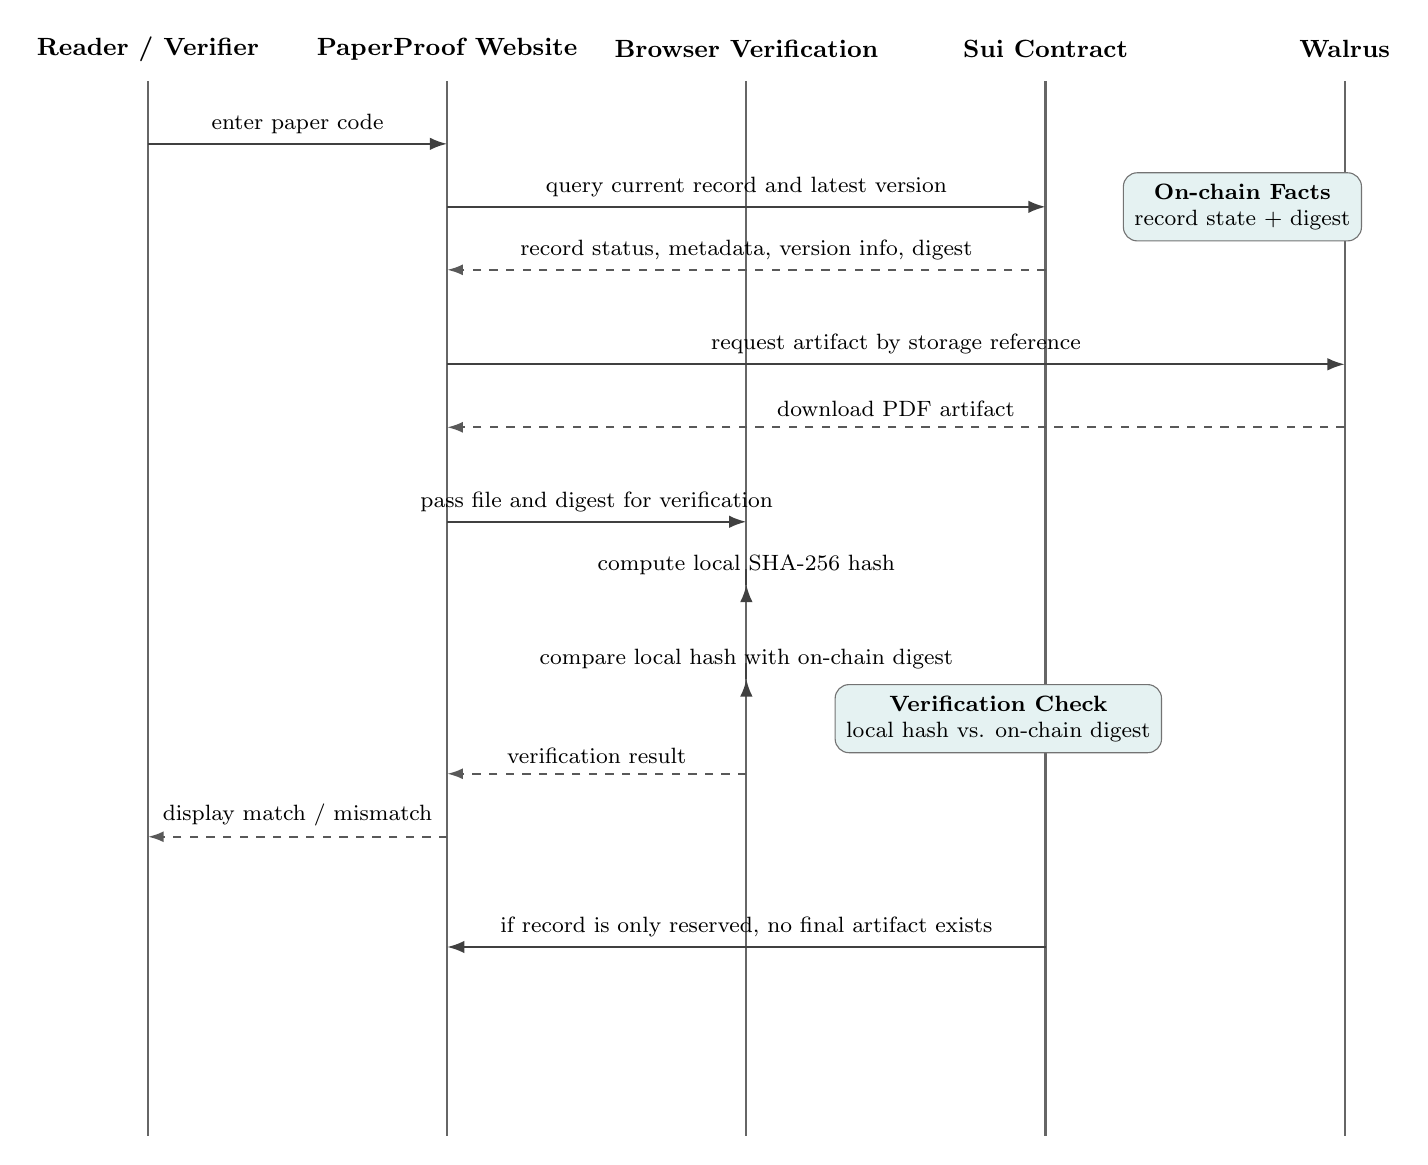
\begin{tikzpicture}[
    font=\small,
    lifeline/.style={draw=black!60, thick},
    msg/.style={-{Latex[length=2.2mm,width=1.6mm]}, thick, draw=black!75},
    reply/.style={-{Latex[length=2.0mm,width=1.4mm]}, thick, dashed, draw=black!65},
    note/.style={
        rectangle,
        rounded corners=4pt,
        draw=black!40,
        fill=gray!8,
        align=left,
        font=\footnotesize,
        inner sep=5pt
    },
    state/.style={
        rectangle,
        rounded corners=5pt,
        draw=black!55,
        fill=teal!10,
        align=center,
        font=\footnotesize,
        inner sep=4pt
    }
]

% =========================================================
% Participants
% =========================================================
\node at (0,0) {\textbf{Reader / Verifier}};
\node at (3.8,0) {\textbf{PaperProof Website}};
\node at (7.6,0) {\textbf{Browser Verification}};
\node at (11.4,0) {\textbf{Sui Contract}};
\node at (15.2,0) {\textbf{Walrus}};

% Lifelines
\draw[lifeline] (0,-0.4) -- (0,-13.8);
\draw[lifeline] (3.8,-0.4) -- (3.8,-13.8);
\draw[lifeline] (7.6,-0.4) -- (7.6,-13.8);
\draw[lifeline] (11.4,-0.4) -- (11.4,-13.8);
\draw[lifeline] (15.2,-0.4) -- (15.2,-13.8);

% =========================================================
% Sequence messages
% =========================================================

% Query by code
\draw[msg] (0,-1.2) -- node[above, font=\footnotesize] {enter paper code} (3.8,-1.2);
\draw[msg] (3.8,-2.0) -- node[above, font=\footnotesize] {query current record and latest version} (11.4,-2.0);
\draw[reply] (11.4,-2.8) -- node[above, font=\footnotesize] {record status, metadata, version info, digest} (3.8,-2.8);

\node[state] at (13.9,-2.0) {\textbf{On-chain Facts}\\record state + digest};

% Retrieve artifact
\draw[msg] (3.8,-4.0) -- node[above, font=\footnotesize] {request artifact by storage reference} (15.2,-4.0);
\draw[reply] (15.2,-4.8) -- node[above, font=\footnotesize] {download PDF artifact} (3.8,-4.8);

% Local verification
\draw[msg] (3.8,-6.0) -- node[above, font=\footnotesize] {pass file and digest for verification} (7.6,-6.0);
\draw[msg] (7.6,-6.8) -- node[above, font=\footnotesize] {compute local SHA-256 hash} (7.6,-6.8);
\draw[msg] (7.6,-8.0) -- node[above, font=\footnotesize] {compare local hash with on-chain digest} (7.6,-8.0);

\node[state] at (10.8,-8.5) {\textbf{Verification Check}\\local hash vs. on-chain digest};

% Return result
\draw[reply] (7.6,-9.2) -- node[above, font=\footnotesize] {verification result} (3.8,-9.2);
\draw[reply] (3.8,-10.0) -- node[above, font=\footnotesize] {display match / mismatch} (0,-10.0);

% Optional reserved-state path
\draw[msg] (11.4,-11.4) -- node[above, font=\footnotesize] {if record is only reserved, no final artifact exists} (3.8,-11.4);

\end{tikzpicture}

\end{document}
